\section{Displasia congenita ossea}

\begin{figure}[!ht]
\centering
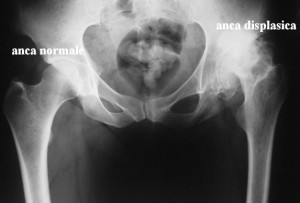
\includegraphics[width=0.4\textwidth]{018/image1.jpeg}
\end{figure}

E' una patologia congenita alla base di un elevato numero di artrosi che arrivano al tavolo operatorio per un trattamento protesico. Patologia quindi che si presenta alla nascita e si riverbera su tutto il percorso della vita fino alla coxoartrosi. L'artrosi si divide in:
\begin{itemize}
\item \textbf{primaria(primitiva)} non esiste una causa ben precisa alla sua origine (il paziente non ha avuto traumi, non ha avuto necrosi da cortisone, non ha la gotta)
\item \textbf{secondaria} (displasia congenita, epifisiolisi, distruzione dell'acetabolo per traumi) c'è sempre una causa ben precisa.
\end{itemize}
\textbf{Un'elevata quota di artrosi secondarie sono secondarie ad una DISPLASIA CONGENITA DELL'ANCA.}

Raramente questa condizione può guarire spontaneamente, mentre molto più frequente è la sua evoluzione attraverso gli stadi di \textbf{sublussazione} e \textbf{lussazione cronica inveterata}. Se non viene diagnosticata alla nascita, in genere diventa chiaramente manifesta con la lussazione favorita dal carico e dalla deambulazione
nell'infante attorno all'anno di età, e nell'adulto questa patologia è un'importante causa di artrosi secondaria.

\subsection{Definizione}

Innanzitutto per:
\begin{itemize}
\item \textbf{\emph{displasia}} intendiamo un difetto di forma e in particolar modo, nel nostro caso, dell'anca, quindi né semplicemente dell'acetabolo, nè semplicemente del femore, ma di entrambi

\begin{figure}[!ht]
\centering
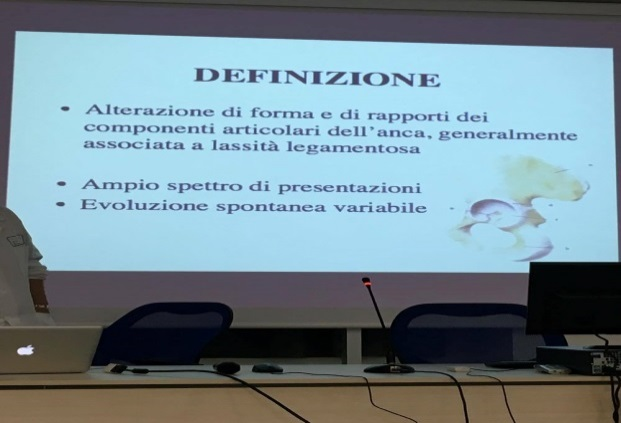
\includegraphics[width=0.4\textwidth]{018/image2.jpeg}
\end{figure}

\item \textbf{\emph{congenita}} perchè esiste una significativa familiarità soprattutto a carico del sesso femminile. Molto spesso infatti c'è una discendenza.
\end{itemize}

Il termine \emph{lussazione dell'anca} è ormai desueto perchè esprime un concetto ben preciso: la testa del femore è fuori dall'acetabolo. Per lussazione infatti si intende una perdita completa dei rapporti articolari che raramente tornano apposto da soli. Spesso tale displasia
è bilaterale.

\subsection{Anatomia patologica}

La coppa acetabolare se invece di essere emisferica ha una parte superiore deformata e quindi è poco coprente tenderà a causare la fuoriuscita della testa femorale soprattutto quando il bambino si alzerà in piedi. \emph{Quindi per displasia congenita dell'anca intendiamo scarsa copertura dell'acetabolo nei confronti della testa}. Si possono
associare delle alterazione a livello del femore:

L'asse cervico-cefalico e quello diafisario si incontrano formando un angolo di 125 gradi ma se le anche presentano un angolo più ampio (130 o 135 gradi) si parla di \textbf{coxa valga}, se invece si riduce \textbf{coxa vara}. Questo è molto importante perchè modifica i carichi
che si realizzano e se, alla displasia che mi determina la presenza di una coppa poco coprente e svasata in alto, aggiungiamo anche una coxa valga, il sistema diventa scivolante e da lì si ha la progressione verso una sublussazione e lussazione.

\begin{figure}[!ht]
\centering
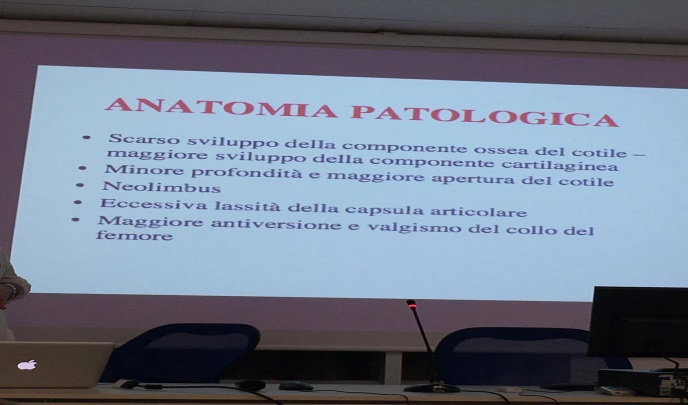
\includegraphics[width=0.4\textwidth]{018/image3.jpeg}
\end{figure}

\begin{figure}[!ht]
\centering
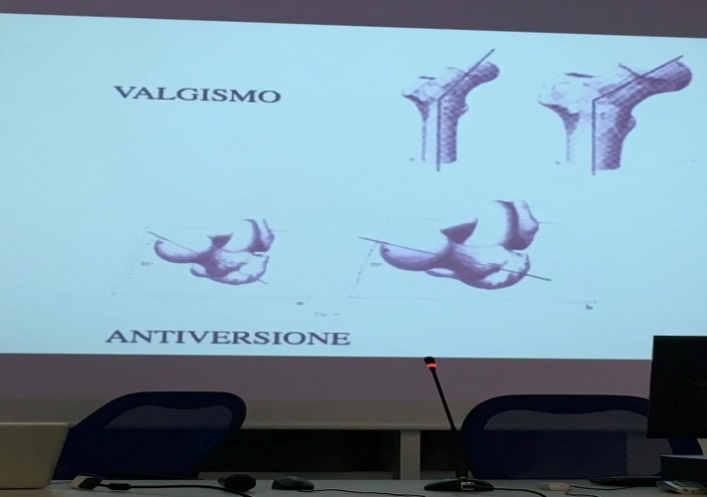
\includegraphics[width=0.4\textwidth]{018/image4.jpeg}
\end{figure}

Tutto ciò quindi comporta (valgo-valgismo) oppure l'antiretroversione (se infatti guardiamo il femore dall'alto, questo non è ortogonale all'asse mediano ma è un po' antiverso. Se il collo è troppo antiverso e tenderà a scoprirsi rispetto all'acetabolo e se è ,anche, valgo-antiverso si scoprirà in alto e in avanti. Infine, quindi, si può dire come il sommarsi di diverse alterazioni morfologiche favoris cano la progressione della malattia displasica. ( un bambino che corre con i piedi in dentro non ha problemi a livello plantare ma probabilmente è un
antiversione dei colli femorali eccessiva e, quindi, quando il bambino tende a centrare le sfere gira i piedi all'indentro e sarà un bambino che molto probabilmentete riuscirà a stare seduto con le gambe all'indietro appoggiato con le ginocchia in quella che è definita TV-position. Se allo stesso bambino gli viene chiesto di sedersi come un indiano non resisterà più di un minuto in quella posizione. La sua antiversione aumenta la possibilità di intrarotazione ma gli limita la possibilità di extrarotazione). Nella coxa normale le forze del carico verranno distribuite su tutta la sfera mentre nella coxa valga si distribuiranno in una sola porzione sviluppando delle artrosi.

\subsection{Presentazione clinica}

La displasia dell'anca si può presentare come:
\begin{itemize}
\item \textbf{semplice displasia} (stadio di pre-lussazione) cioè come una coppa poco corrente ma rapporti mantenuti tra acetabolo e testa. Si estende in genere fino al decimo mese di vita. Morfologicamente e radiologicamente, l'acetabolo si presenta ovalizzato, e nella sua porzione postero-superiore si può osservare una piccola salienza smussata, nota come \emph{neolimbus}, formato da cartilagine articolare, accolto in una \emph{introflessione del ciglio cotiloideo}.
\item \textbf{testa che è un po' risalita} (stadio di sublussazione) e tende quasi ad uscire dall'acetabolo deformando il cercine fibrocartilagineo, stirando il legamento rotondo e la capsula.
Si manifesta solitamente dopo i 10 mesi di vita sino ai 10 anni di età, raramente presente alla nascita (se infatti fosse presente alla nascita, bisognerebbe ricercare ulteriori malformazioni).
\item \textbf{completamente fuorisede} (stadio di lussazione) e parleremo di lussazione congenita dell'anca. Il momento in cui questa lussazione comparirà sarà quando ad un anno di vita circa il bimbo si mette in piedi.
\end{itemize}

Questi ultimi stadi si instaurano nel tempo come evoluzione naturale di una pre-lussazione non trattata ed è caratterizzata dalle seguenti alterazioni:

\begin{itemize}
\item
  \textbf{Alterazioni Osteo-Cartilaginee}: La testa del femore è dislocata nella fossa iliaca esterna, al di sotto dei muscoli glutei, con il neocotile che è in comunicazione con una doccia di migrazione con l'acetabolo, il quale, non essendo sottoposto allo stimolo pressorio della testa del femore, presenta un'ipoplasia della cartilagine ed un'ipertrofia del tessuto fibro-adiposo, detto pulvinar.
\item
  \textbf{Alterazioni Capsulo-Legamentose}: Il legamento rotondo si presenta allungato ed ipertrofico, così come il legamento trasverso dell'acetabolo, ed il cappuccio pericefalico della capsula è ispessito. Tutti questi elementi sono ostacoli meccanici ed anatomici alla riduzione della testa del femore nell'acetabolo.
\item
  \textbf{Alterazioni Muscolo-Tendinee}: I muscoli adduttori e l'ileo-psoas sono accorciati ed il tendine del secondo strozza la capsula articolare, deformandola a forma di clessidra.
\end{itemize}

\subsection{Epidemiologia e eziopatogenesi}

L'incidenza è di 4 su 1000, 5-8:1 F:M. Bilaterale nel 45 \% dei casi.

\textbf{Fattori genetici} sono dimostrati dalla presenza di:
\begin{itemize}
\item \emph{Familiarità}
\item \emph{Elevata frequenza nei gemelli omozigoti}
\item \emph{Frequente associazioni con altre alterazioni congenite (PTC, TORCICOLLO CONGENITO)}
\item \emph{Prevalenza nel sesso femminile}
\item \emph{Prevalenza nella razza bianca}
\end{itemize}

Inoltre vi sono i \textbf{fattori ambientali}, dati da:
\begin{itemize}
\item SPAZI RISTRETTI SOPRATTUTTO IN GRAVIDANZA
\item DISPOSTURE INTRAUTERINE OBBLIGATE
\item ATTEGGIAMENTI NEONATALI ORMAI ABBANDONATI NELLE NOSTRE TRADIZIONI
(Bambini fasciati con le gambe strette quasi come mummie. Questa posizione è l'esatto contrario di quella che si fa assumere in terapia)
\item OLIGOIDRIAMNIOS
\end{itemize}

Per quanto riguarda l'EZIOPATOGENESI, sono state fatte diverse ipotesi per giustificare lo sviluppo della displasia dell'anca: la prima ipotesi prevede la possibile presenza di \textbf{\emph{vizio di posizione fetale}}, e infatti la patologia è più comune in caso di primogenitura o di presentazione podalica, mentre secondo la \textbf{\emph{teoria}} \textbf{\emph{della displasia acetabolare}} la causa risiederebbe in una debolezza della cartilagine acetabolare, che sarebbe quindi meno resistente alle sollecitazioni meccaniche della testa del femore, col risultato di dare un rapporto anatomico anomalo. Infine abbiamo anche la \textbf{\emph{teoria della lassità capsulo-legamentosa}}, in base alla quale la struttura di contenizione passiva dell'articolazione conterrebbe una maggior quota di fibre elastiche, per cui non riuscirebbe ad indirizzare correttamente lo sviluppo reciproco dei due capi articolari. Le varie ipotesi non si escludono a vicenda, anzi è probabile che i vari fattori si combinino tra loro determinando lo sviluppo della patologia, come ipotizzato dall'\textbf{ipotesi di Wynne-Davies}, in base alla quale la displasia congenita dell'anca sarebbe una patologia a trasmissione multigenica, evolutivamente favorita dal passaggio alla statura eretta, e che potrebbe peraltro essere connessa con diversi polimorfismi del recettore per l'ormone \emph{relaxina}, normalmente prodotto dalla madre al termine della gravidanza, e che determina una diastasi della sinfisi pubica per facilitare il passaggio del feto nel canale del parto.

\subsection{Diagnosi}

Quanto più è precoce possibile tanto migliore sarà il successo del trattamento.

Il primo segno clinico per fare diagnosi è:

\begin{itemize}
\item
  \textbf{l'anamnesi} (ad, esempio, femmina, figlia di displasici o nipote di dispasici).
\item
  \textbf{esame clinico}

\begin{figure}[!ht]
\centering
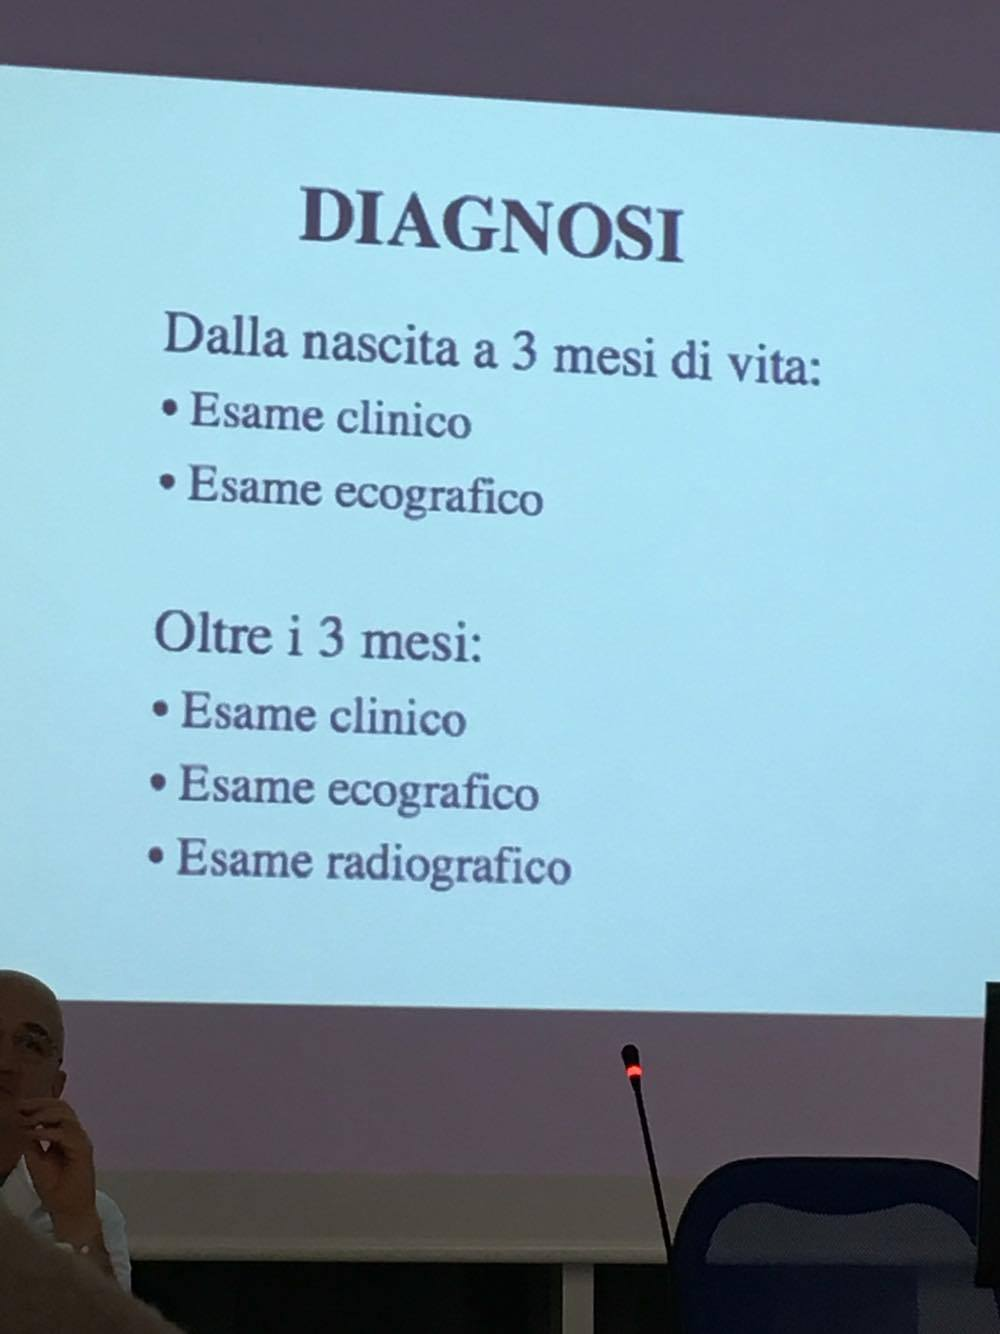
\includegraphics[width=0.4\textwidth]{018/image5.jpeg}
\end{figure}

\item
  \textbf{ecografia }
\item
  \textbf{radiografia} verso il 3 mese, ma se ci sono dei sospetti si anticipa.
\item
  il bambino deve essere visitato dal \textbf{neonatologo e dal pediatra} che individueranno i seguenti segni:
\end{itemize}

\textbf{\emph{Esame clinico:}}

\begin{figure}[!ht]
\centering
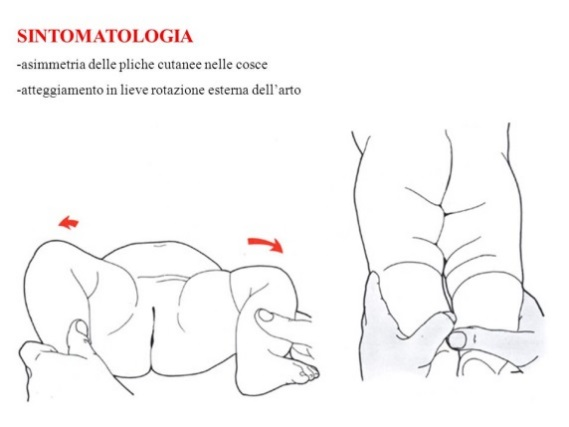
\includegraphics[width=0.4\textwidth]{018/image6.jpeg}
\end{figure}

\begin{itemize}
\item[1.] Durante  il primo mese di vita si ha un segno molto particolare che è \emph{lo \textbf{scatto di ortolani}}
\item[2.] si riscontra, inoltre, un \textbf{\emph{DEFICIT DI ABDUZIONE delle anche}}

L'\emph{abduzione è limitata} e l'andatura presenta una zoppia da caduta di bacino conseguente sempre all'ipotrofia dei glutei (\textbf{fenomeno di Trendelenburg}), mentre se la displasia è bilaterale la marcia è anserina.

\item[3.] \textbf{asimmetria delle pliche cutanee}

\item[4.] \textbf{accorciamento del femore apparente} ( perchè in realtà non è accorciato ma è uscito dall'acetabolo). Il bambino perciò dopo la nascita lo si deve osservare e sollecitare per vedere come muove le
gambe: devono muoversi nello stesso modo, infatti, se una scalcia e l'altra no, c'è qualcosa che non va.
\end{itemize}

\emph{La \textbf{manovra dello scatto di Ortolani}} si fa in bambini di età inferiore al mese e consiste in un movimento come se si volesse riportare in sede la testa fuori sede; oppure per gli anglosassoni il 'Barlow', da noi chiamato 'il segno inverso di ortolani', dove lo si
porta fuori (vedi immagine).

\emph{\textbf{Deficit dell' abduzione}:} quando noi mettiamo un bambino su un piano e gli apriamo le gambe, le ginocchia devono arrivare quasi a toccare il piano, normalmente. Soprattutto se si nota che una gamba si apre bene e l'altra no, quella che non si apre bene è fortemente sospetta di una displasia congenita.

\begin{figure}[!ht]
\centering
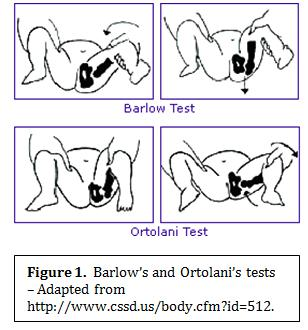
\includegraphics[width=0.4\textwidth]{018/image7.jpeg}
\end{figure}

\begin{figure}[!ht]
\centering
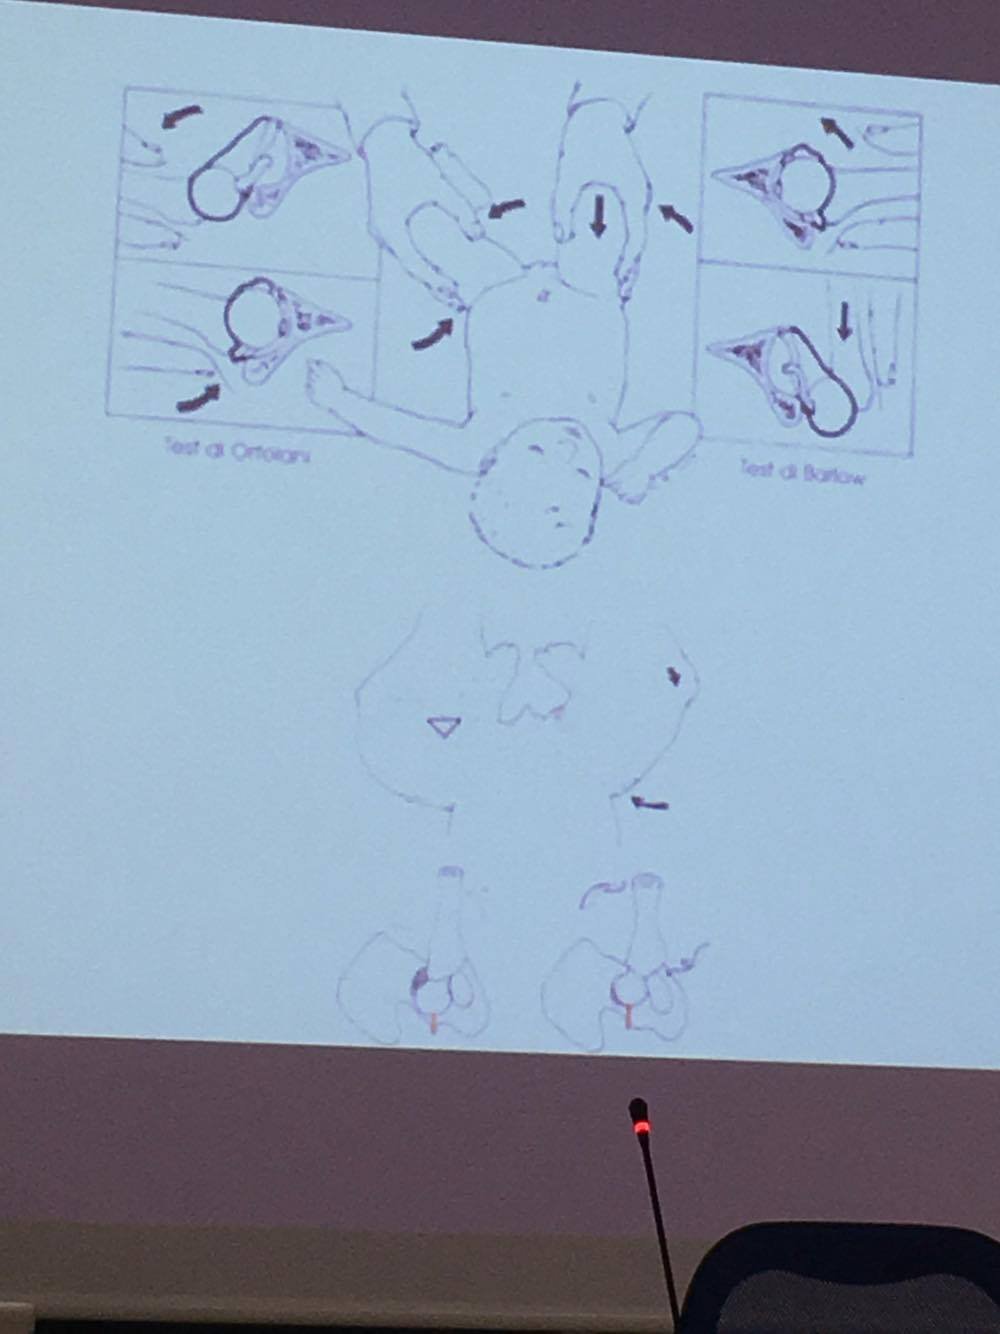
\includegraphics[width=0.4\textwidth]{018/image8.jpeg}
\end{figure}

\emph{\textbf{L'asimmetria delle pliche cutanee}} è un segno molto valido, indice di notevole gravità, vuol dire che l'anca è uscita dall'acetabolo già nel primo mese, per cui le pliche non sono coincidenti. Si tratta di un'asimmetria significativa che poi si associa a dei deficit di abduzione.
\\\\
\textbf{\emph{Esame ecografico}}: Fin dagli anni 80, Graft, radiologo austriaco, introduce il concetto di ecografia dell'anca infantile perchè questa metodica diagnostica ha la capacità di studiare i tessuti che in
quell'epoca di vita non sono calcificati e rispetto ad una radiografia presenta grossissimi vantaggi:
\begin{itemize}
\item non è dannosa ( no radiazioni)
\item ha una significatività molto precoce rispetto alla radiografia poichè per dare informazioni significative non deve aspettare il 4-5 mese, quando si comincia ad avere calcificazione ossea in quanto studia quello che non è osseo. Al 4-5 mese una radiografia potrà farci vedere bene come è fatta l'anca dal punto di vista osseo, ma non darà mai informazioni sulla copertura data dal cercine fibrocartilagineo.
\end{itemize}

Graft ha diviso la lesione in 4 gradi in base all'ecografia:

\begin{figure}[!ht]
\centering
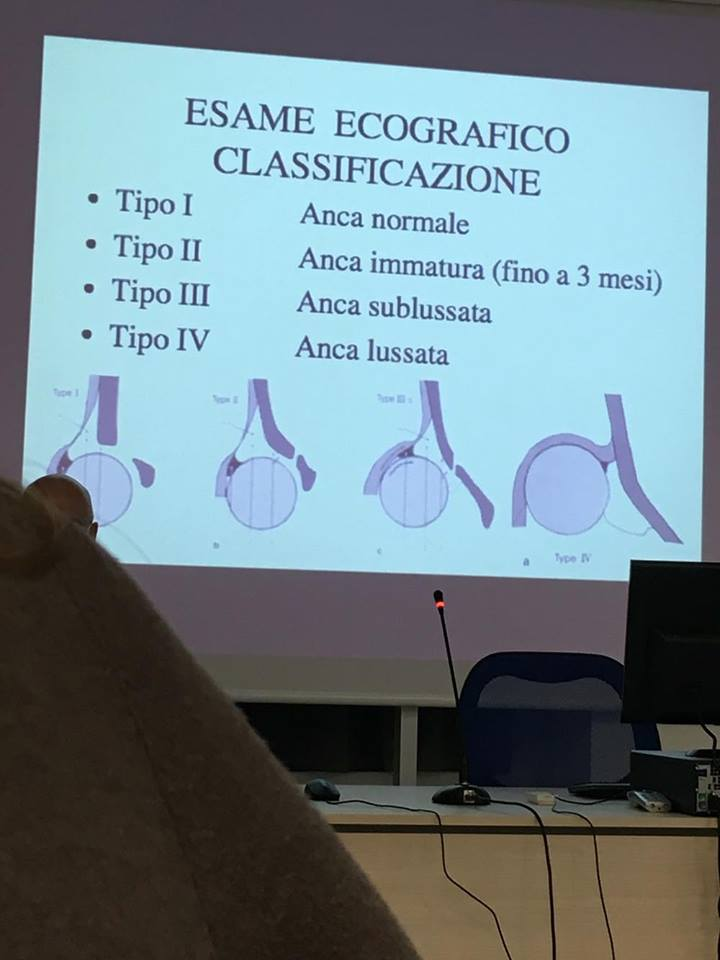
\includegraphics[width=0.3\textwidth]{018/image9.jpeg}
\end{figure}

La componente cartilaginea si continua con il cercine fibrocartilagineo, quello che sarà poi il \emph{labrum acetaboli}. Quindi, la testa in un anca normale è circondata da osso, cartilagine, fibrocartilagine che ricopre il tutto.

Nella displasia c'è un anca che possiamo definire \emph{immatura} ma che tendenzialmente dovrebbe maturare, in cui la componente ossea è svasata, non più ben angolata. È immatura perchè in realtà c'è una copertura totale da parte della componente cartilaginea e fibrocartilaginea; quindi è un anca che maturerà in senso positivo. (siamo ottimisti quando ci troviamo davanti ad un tipo 2 secondo graft.)

nel tipo 3 invece è diverso, perchè diventa insufficiente anche la componente cartilaginea; si arriva fino al grado 4, poi ci sono delle sottoclassi.

\begin{figure}[!ht]
\centering
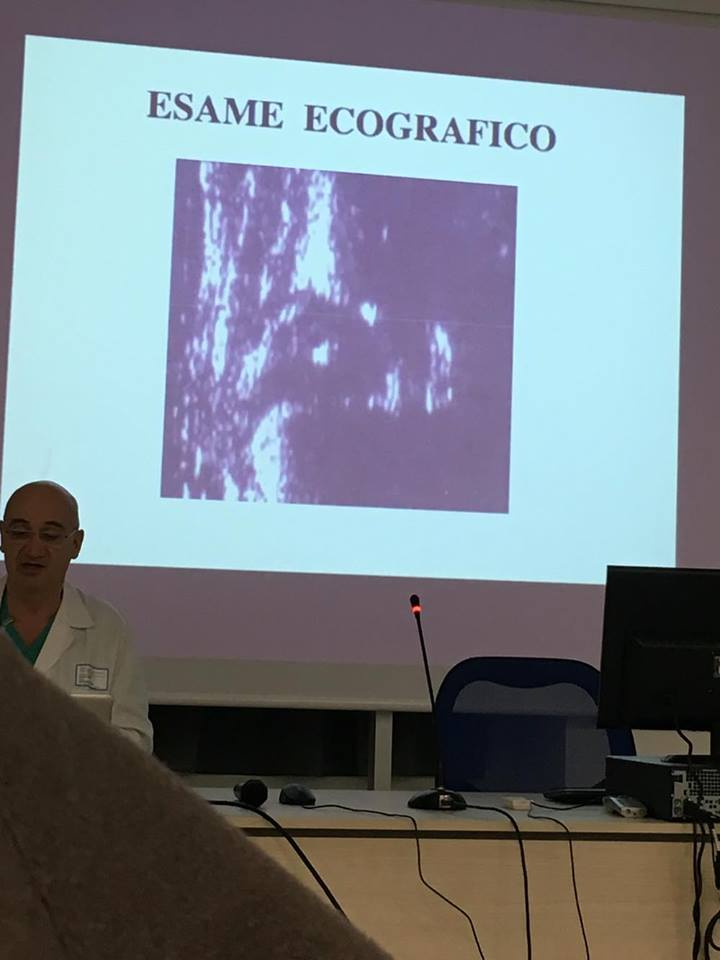
\includegraphics[width=0.3\textwidth]{018/image10.jpeg}
\end{figure}

Il prof. mostra un'ecografia e indica la testa del femore, il nucleo cefalico, la componente ossea e cartilaginea, il labrum acetabuli, i muscoli pelvici-trocanterici. Vedendo quest'eco si deduce che la copertura è buona, il nucleo è sviluppato e ben centrato.
\\\\
\textbf{ANCA SUBLUSSATA}: \emph{Il cercine fibrocartilagineo si fa estroflettere e non contiene più la testa}, mentre la \emph{capsula e il legamento rotondo sono stirati}. E' un anca che soffre e quindi anche il nucleo di ossificazione non compare oppure è ipoplasico rispetto a quello controlaterale ammesso che non si tratti di una forma bilaterale. Questa forma poi evolve verso la lussazione vera e propria.

\begin{figure}[!ht]
\centering
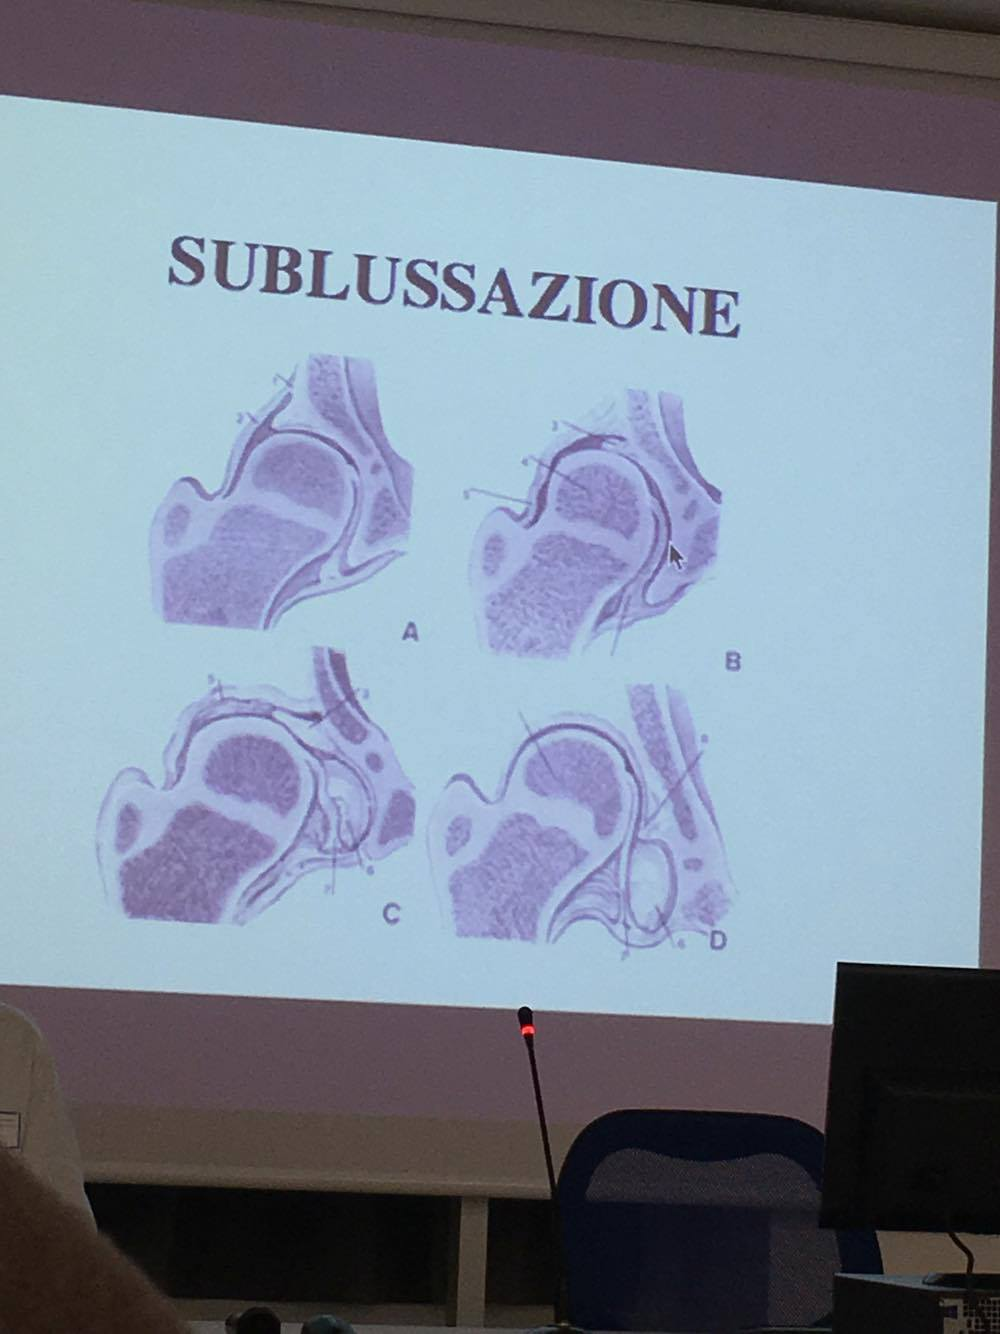
\includegraphics[width=0.3\textwidth]{018/image11.jpeg}
\end{figure}

\textbf{LUSSAZIONE}: si ha la capsula che stringe come l'istmo di una clessidra, mentre il \emph{legamento rotondo} e il \emph{tendine dell'ileo psoas} vanno a ghigliottinare l'istmo della clessidra impedendo all'ortopedico di riposizionare con un gesto terapeutico la testa del femore. La lussazione poi ha dei gradi di evoluzione e può arrivare alla lussazione iliaca cioè la testa si va a porre nella muscolatura glutea.

\begin{figure}[!ht]
\centering
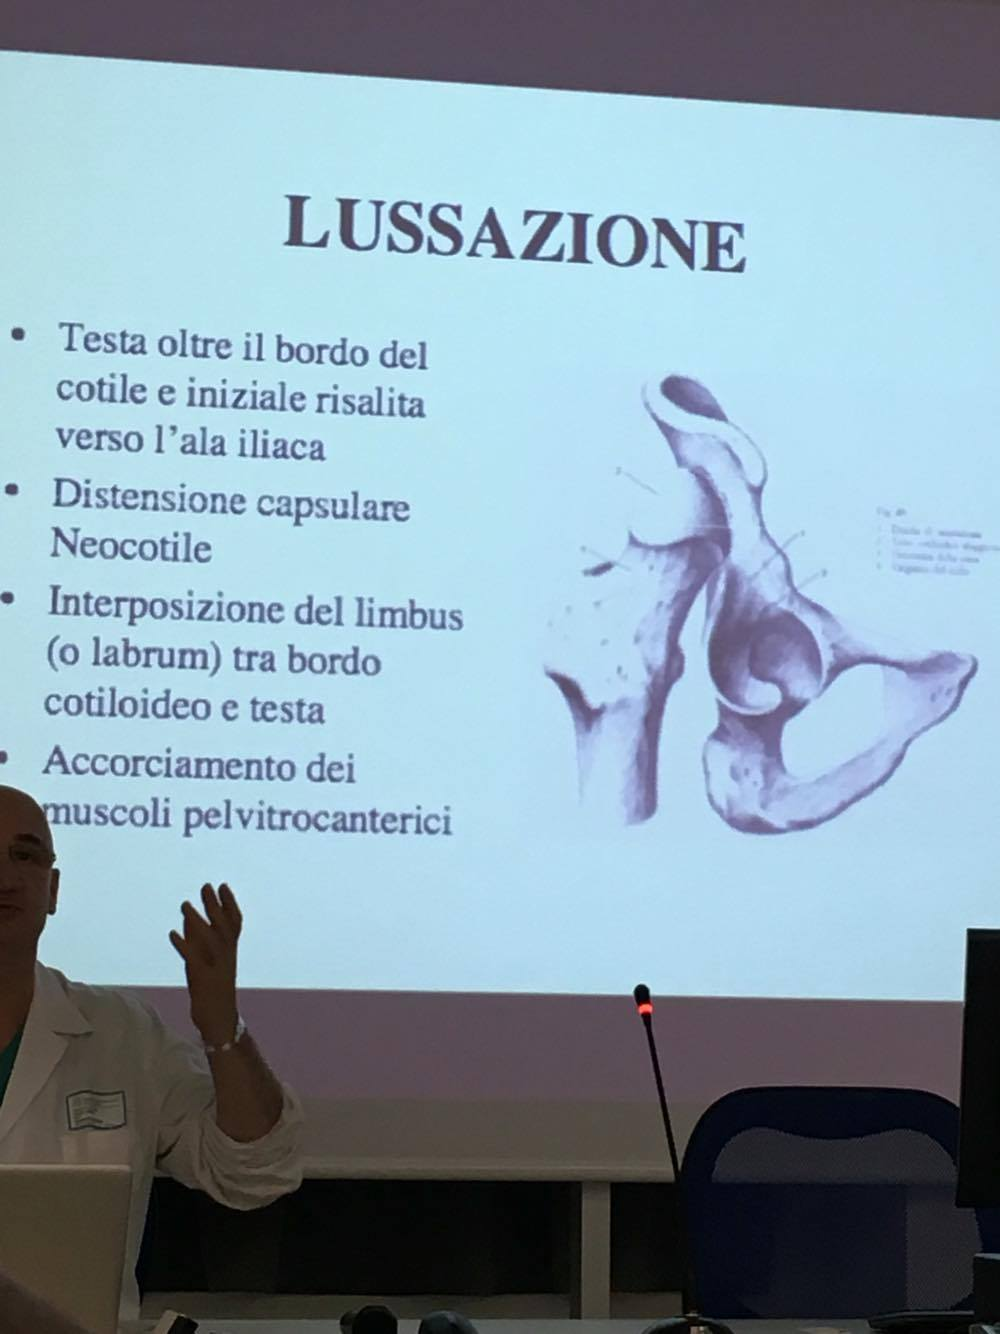
\includegraphics[width=0.3\textwidth]{018/image12.jpeg}
\end{figure}

L'eco inoltre è un esame non invasivo, ripetibile, evidenzia le parti molli e tutti i componenti delle articolazioni, è estremamente sensibile, permette di controllare l'evoluzione degli effetti del trattamento, è valido nel neonato per tutto il primo anno, dopodichè
l'acetabolo diventa troppo sostituito da osso e quindi non riesce più a dare una risposta significativa

\textbf{Ci sono delle sottoclassi di pertinenza del pediatra o radiologo}.

\textbf{\emph{Esame radiografico}}: diventa significativo al 4-5 mese quando compare il nucleo di ossificazione. Si vede un immagine di una sublussazione molto grave dove si interrompe \emph{\textbf{l'arco di Shenton}} che si traccia dal margine interno del femore fino al margine
superiore del forame otturato (ad arco romano). In displasia questo arco viene interrotto.

La \emph{\textbf{\emph{triade di Putti}}} è data da dei segni molto importanti quasi sempre presenti assieme:
\begin{itemize}
\item \textbf{Inclinazione dell'acetabolo} ( non è 30 gradi, ma sale a 40-45 diventando poco coprente e sfuggente).
\item \textbf{Assenza o ipoplasia del nucleo cefalico. }
\item \textbf{Tirando una linea che passa attraverso le cartilagini psiloniche e che scende attraverso il margine acetabolare si definisce un incrocio di linee all'interno del quale la testa sana si trova ad essere esattamente all'interno dell'incrocio mentre la testa malata
sarà ipoplasica, lateralizzata e risalita rispetto alla forma normale.}
\end{itemize}

Esame radiografico (immagine) ==\textgreater{} arco di Shenton interrotto, nucleo ipoplasico e insufficiente
copertura acetabolare.

\begin{figure}[!ht]
\centering
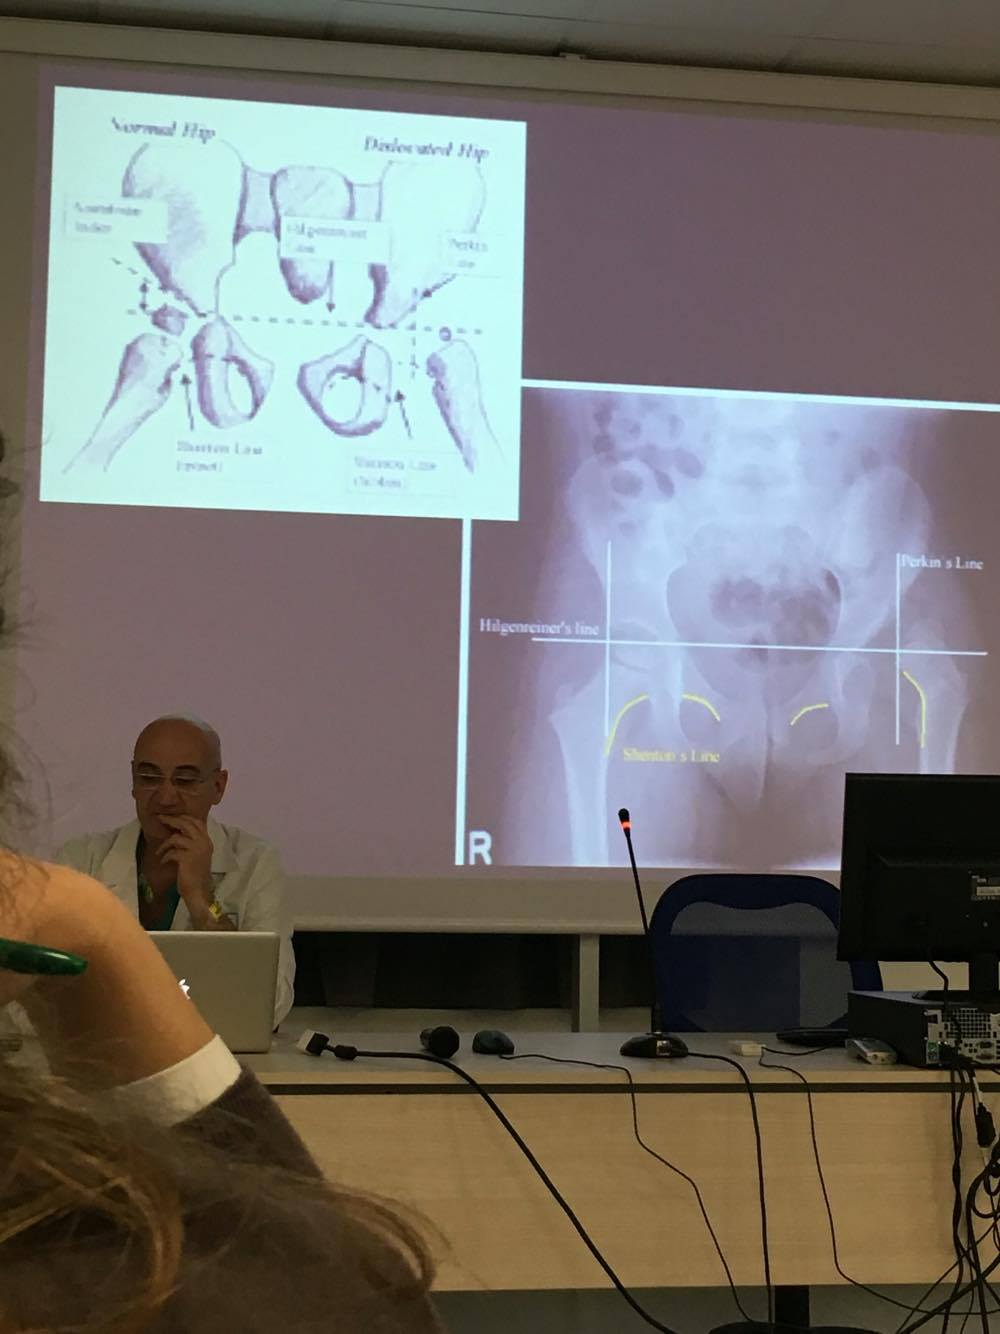
\includegraphics[width=0.3\textwidth]{018/image13.jpeg}
\end{figure}

\begin{figure}[!ht]
\centering
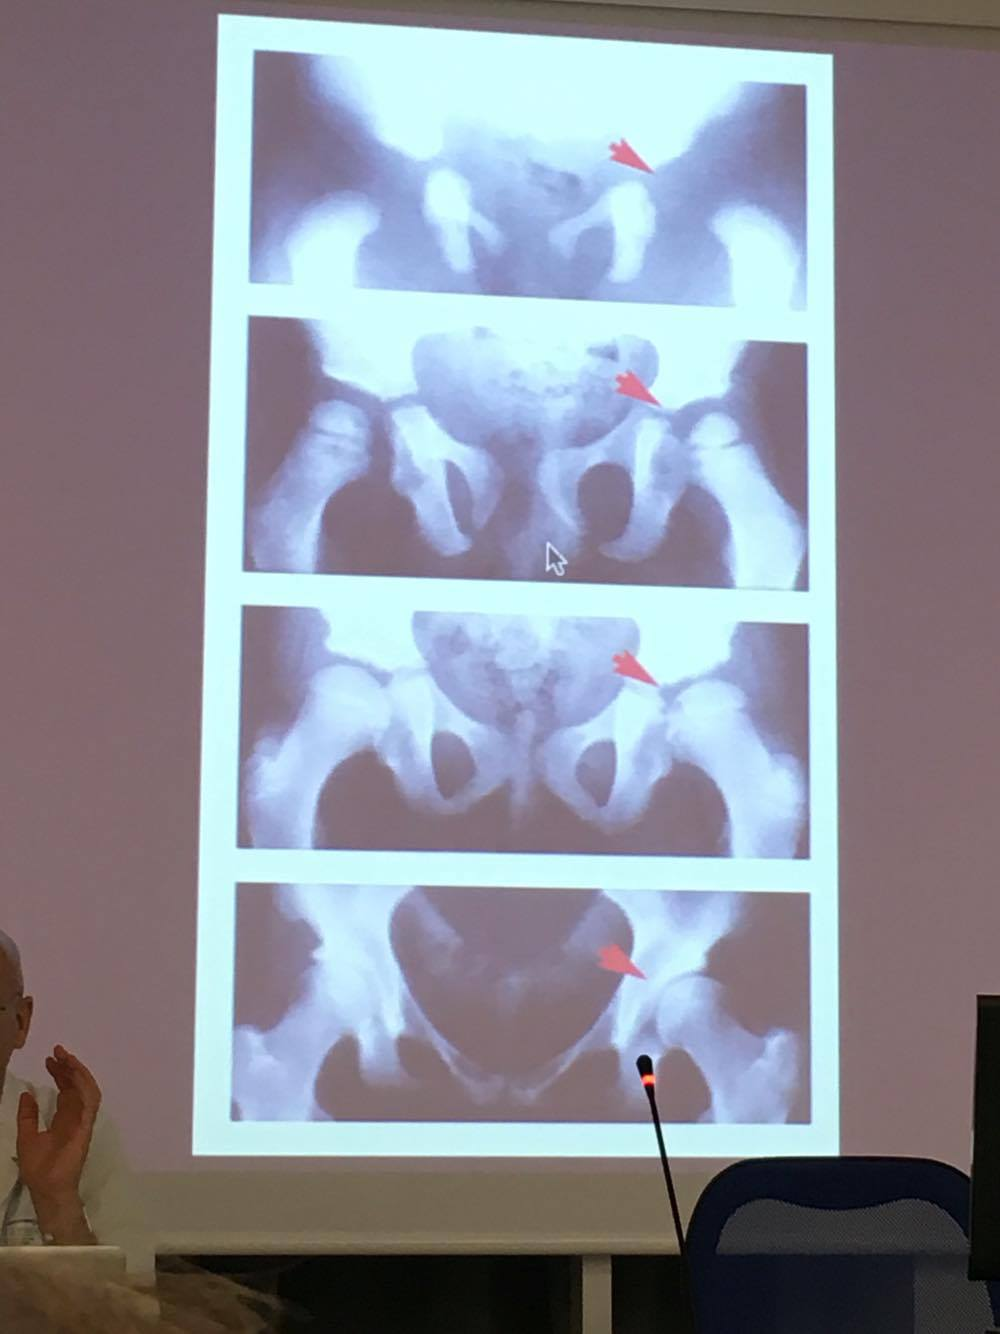
\includegraphics[width=0.3\textwidth]{018/image14.jpeg}
\end{figure}

\subsection{Trattamento}

Più è precoce, migliore è il risultato. I risultati cambiano se si interviene entro i primi 3 mesi o entro l'anno.

Principi di trattamento:

\begin{itemize}
\item
  \textbf{mantenere le anche in una posizione di abuduzione e flessione}: in tale posizione metteremo la testa che tendeva ad uscire dentro il cotide, lo scopo è far si che il cotide si modelli, crescendo, intorno alla testa e recuperi la sua azione di copertura.
\item
  Le gambe vengono tenute in posizione grazie a dei \textbf{tutori di varia forma}, in modo statico o dinamico (con delle \emph{bretelle} che consentono di flettere o abdurre l'anca, ma non di estenderla o addurre).
\item
  Non è sufficiente mettere il \emph{doppio pannolone}, poichè questo può andar bene solo in quelle anche immature, anche se oggi si usa abitualmente la \emph{'mutandina di Giò'} che mantiene l'apertura delle gambe un po' di più di quanto faccia il doppio pannolone e un po' meno del \emph{doppio divaricatore}.
\item
  \emph{Per \textbf{quanto tempo} si tengono nell'arco della giornata e per quanto tempo si tengono nel tempo?} Si tengono 24h su 24, si tolgono soltanto per l'igiene intima, per il bagnetto, fino a quando gli esami eco-radiografici non mostrano che si è sviluppato in modo armonico il rapporto tra testa e acetabolo. Orientativamente non si va sotto i 4 mesi.(domanda d'esame)
\item
  Quando invece le forme sono gravi non è sufficiente mettere il divaricatore. La testa del femore sublussata è fuorisede. Non è possibile rimetterla in sede se non tramite una trazione progressiva che riduca la testa dentro l'acetabolo e successivamente tramite l'utilizzo di apparecchi gessati che vanno rinnovati poichè i bambini crescono e vanno mantenuti fino a quando non si vede un buon sviluppo osseo.
\item
  Quando invece l'anca è già lussata alla nascita ed è impossibile ridurla anche con manovre, bisogna fare terapia chirurgica per posizionare la testa in sede.
\item
  È importante trattare le anche, perchè se non trattate si arriva ad una displasia congenita dell'adulto in una forma ancora più grave e ciò comporta una notevole limitazione del movimento dell'anca nella vita quotidiana ed una notevole difficoltà di trattamento chirurgico protesico.
\item
  Nella displasia dell'anca non esiste solo un trattamento nel primo anno di vita, ma anche per le forme più tardive che sono sfuggite. (\textbf{osteotomia pelvica})
\item
  Se abbiamo un cotide poco coprente perchè verticale possiamo fare delle \textbf{osteotomie}, cioè sezione dell'osso di copertura e trazioni per ridurre il femore nel cotile originario ed ottenere una solida anchilosi ossea dell'anca in posizione fisiologica.
\item
  Se abbiamo un'anca troppo valga potremo fare una osteotomia che tende a centrare l'anca; molto spesso i gessi sono associati. Nei casi più gravi ed avanzati, tuttavia, vi è indicazione per procedere con l'impianto di un'\textbf{artroprotesi totale d'anca}
\end{itemize}

\begin{figure}[!ht]
\centering
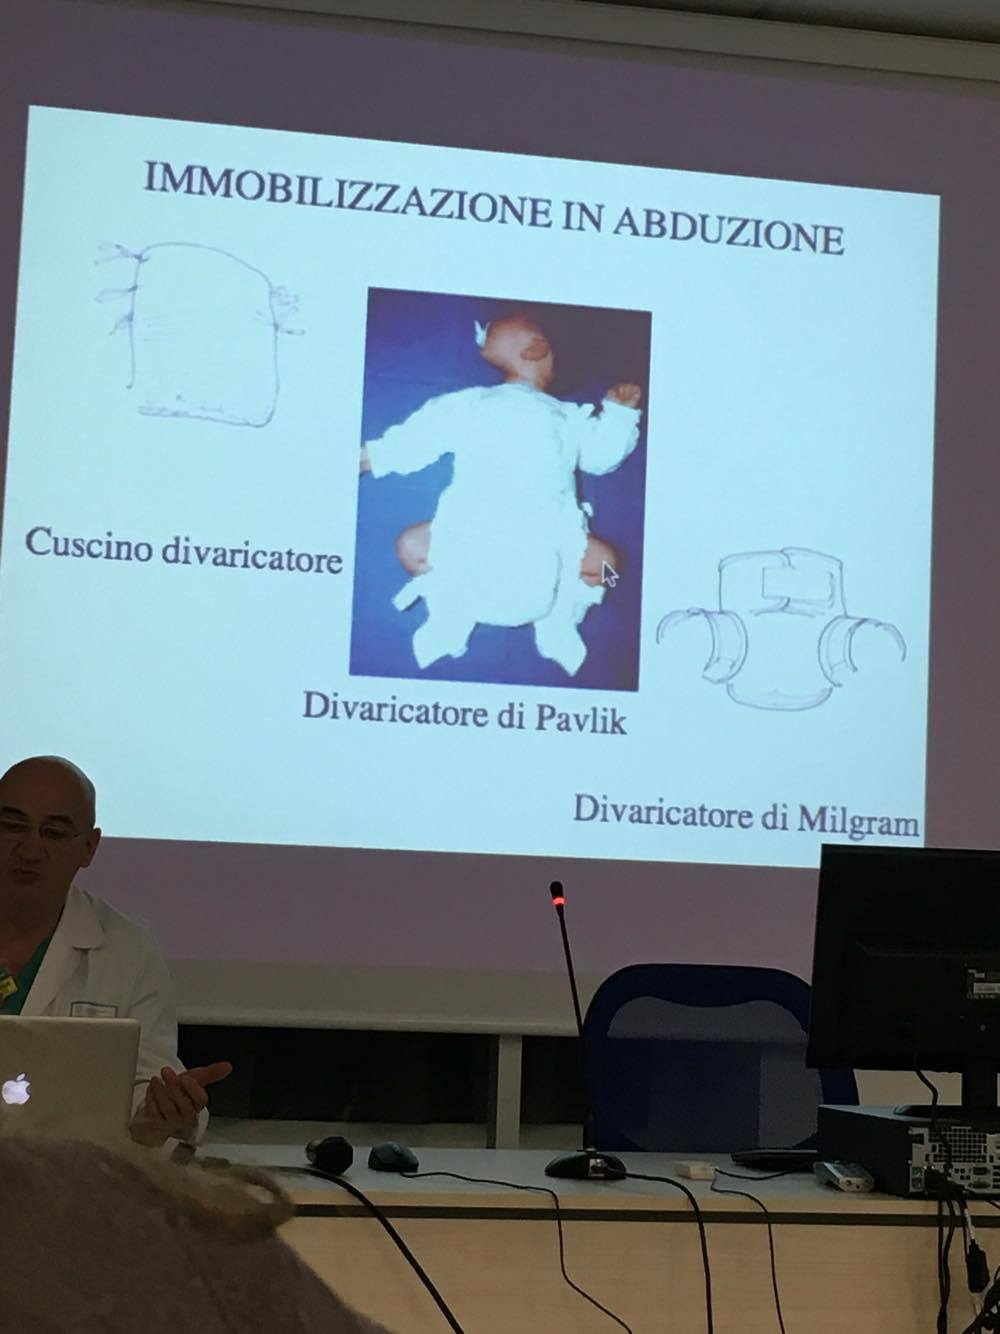
\includegraphics[width=0.3\textwidth]{018/image15.jpeg}
\end{figure}

\begin{figure}[!ht]
\centering
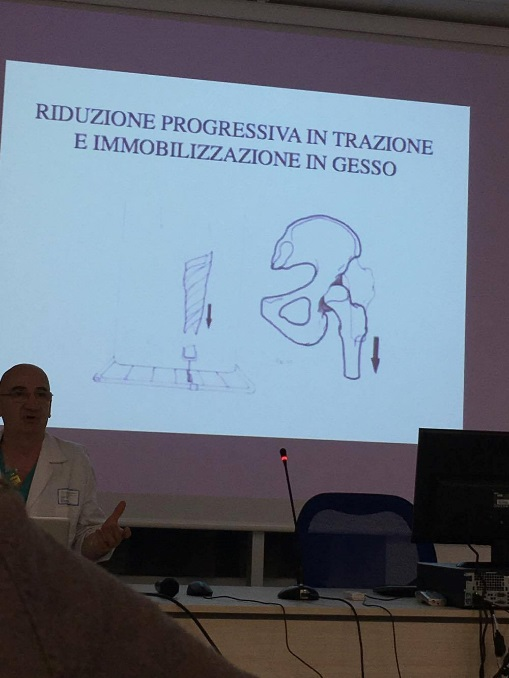
\includegraphics[width=0.3\textwidth]{018/image16.jpeg}
\end{figure}
